\chapter*{Dynamical Systems}

\section*{Fingerprints of Complex Systems}

\begin{itemize}
    \item Multi-agent / multi-component
    \item Decentralized
    \item Local interactions
    \item Dynamic
\end{itemize}

\section*{Types of Abstract Models:}

\begin{description}
    \item[Agent-based] Mechanistic implementation of the multi-component interactions.
    \item[Mathematical (white-box)] Formally describe the relations among the relevant components.
    \item[Black-box] Input-output pairs from the system are used to predict...
    \item[Statistical] Describing patterns and correlations between variables.
\end{description}

\section*{Systems of ODEs}

Here is a system of $n \ge 1$ Ordinary Differential Equations
\[
\begin{cases}
\frac{dx_1}{dt} = f_1(\xx(t))\\
\frac{dx_2}{dt} = f_2(\xx(t))\\
\vdots \\
\frac{dx_n}{dt} = f_n(\xx(t))
\end{cases}
\]
where $\xx(t)$ is an $n$-dim vector.


A continuous-time Dynamical System is defined by a system of differential equations:
\[
\frac{d\xx(t)}{dt} = \mathbf{f}(\xx, t; \theta) \quad \text{or} \quad \dot{\xx} = \mathbf{f}(\xx, t; \theta)
\]
where $\mathbf{f}: \Rn \to \Rn$ specifies how each component of the state evolves as $t$ changes.
It can depend on a set of given parameters $\theta$

\textbf{Some definitions:}

\begin{itemize}
    \item Initial conditions: where the system is at the beginning of the evolution:
    $\xx(t_0)$
    \item Phase space: space of all possible states
    \item Trajectory: the curve traces by $\xx(t)$ in the phase space starting from $\xx(t_0)$
    \item Solution: is in the form $\xx(t; t_0)$ that defines a family of time trajectories
    in the phase space. Once we fix $t_0$, we fix a unique trajectory
\end{itemize}

\section*{Vector fields and flows}
How are solutions built? At any point, $\mathbf{f}$ assigns a vector
that shows where the point is heading (direction of motion).

If we plot these arrows (vectors) in the phase space, we get can
get an idea of how the system evolves.

\textbf{Flow: } $\Phi: \mathtt{R} \times \Rn \to \Rn$ is the collection of
all trajectories generated by all possible starting conditions.

$\Phi(t, \xx_0) = \xx(t; \xx_0)$


A fundamental theorem guarantees
that \textbf{two orbits corresponding to two different initial solutions never intersect with
each other }, except at equilibrium

\section*{Basic Properties}

An ODE is linear if
\begin{itemize}
    \item $\mathbf{f}(\xx) = A\xx$ (Homogeneous)
    \item $\mathbf{f}(\xx) = A\xx + b$ (Affine)
\end{itemize}

Linear ODE enjoys closed form solutions, non-linear ODEs usually not


A system is autonomous if time doesn't appear in expression of $\mathbf{f}$.

Facts:
\begin{itemize}
    \item Any $n$-order ODE can be rewritten as a system of $1$st order ODEs in $\Rn$
    \item Any Non-Autonomous ODE can be rewritten as an autonomous one
\end{itemize}

So we will focus on 1st order, autonomous and linear ODEs

\section*{Solving!}
\begin{center}
    
\includegraphics[width=0.2\textwidth]{images/cat.png}
\end{center}

General form of linear ODE:
\[
\dot\xx = A \xx, \quad x \in \Rn
\]

A solution is a function $\xx(t)$ that satisfies the vector field $A$.

(Lots of derivation out is skipped, here's how to solve)

\begin{enumerate}
    \item Solve $\det(A - \lambda I) = 0$ for $\lambda$
    \item The roots $\lambda_i$ are eigenvalues of $A$
    \item For each $\lambda_i$, there exists a non-null eigenvector
    $\uu_i$
    \item Together they yield one solution: $\xx(t) = \uu_i e^{\lambda_i t}$
    \item Each distinct eigen-pair gives ONE independent vector solution
    \item The general solution is then the combination of these terms:
    $\xx(t) = c_1 e^{\lambda_1 t} \uu_1 + \dots + c_n e^{\lambda_n t} \uu_n$ (at most n terms)
\end{enumerate}

Important: the above is strictly true only if all eigenvalues are distinct

Matrix Exponential representation: $\xx(t) = e^{A t} \xx(0)$ where $\xx(0)$ is a generic initial condition

\section*{Exponentials and Asymtotic Behavior}

Since the solution is a sum of exponentials, stuff is being pulled in the direction of the eigenvectors,
weighted by their corresponding signed eigenvalues.


If the real part of $\lambda_i > 0$, mode $i$ is unstable/diverging.

If the real part of $\lambda_i < 0$, mode $i$ is stable/contracting.

At each point, the solution \textbf{mixes} the modes.

\section*{Equilibrium points}

A state $\xx_e$ is an equilibrium state of a system $\dot\xx = \mathbf{f}(\xx)$ if
when at a time $t_0$ the sytem is at $\xx_e$ then it stays there FOREVER

Why? Velocity of the field in $\xx_e$ is null: $\mathbf{f}(\xx_e) = 0$


For a linear ODE, the equilibrium points are the points of the \textbf{Null Space} (solutions to $A \xx = 0$)
Theres one trivial solution at $\xx = \0$ if $A$ is invertible, o.w. inifnitely many solutions

\section*{Taxonomy of equilibria}

\begin{table}[h!]
\centering
\renewcommand{\arraystretch}{1.3}
\setlength{\tabcolsep}{8pt}
\begin{tabular}{>{\bfseries}m{3.5cm} m{6cm} m{5cm}}
\textbf{Equilibrium Type} & \textbf{System’s Behavior} & \textbf{Trajectories} \\
\midrule
Equilibrium state &
If at or arrives at $\mathbf{x_e}$, it stays at $\mathbf{x_e}$ &
Trajectory is constant: $\mathbf{x}(t) = \mathbf{x_e}$ \\

Stable equilibrium (Lyapunov) &
If started close to $\mathbf{x_e}$, stays close to $\mathbf{x_e}$ forever &
Nearby trajectories remain in a neighborhood of $\mathbf{x_e}$ \\

Asymptotically stable equilibrium &
If started close to $\mathbf{x_e}$, stays close to $\mathbf{x_e}$ and moves toward $\mathbf{x_e}$ as $t \to \infty$ &
Nearby trajectories converge to $\mathbf{x_e}$ \\

Unstable equilibrium &
Even if started very close to $\mathbf{x_e}$, eventually diverges from $\mathbf{x_e}$ &
Nearby trajectories diverge from $\mathbf{x_e}$ \\
\bottomrule
\end{tabular}
\end{table}

\begin{center}
    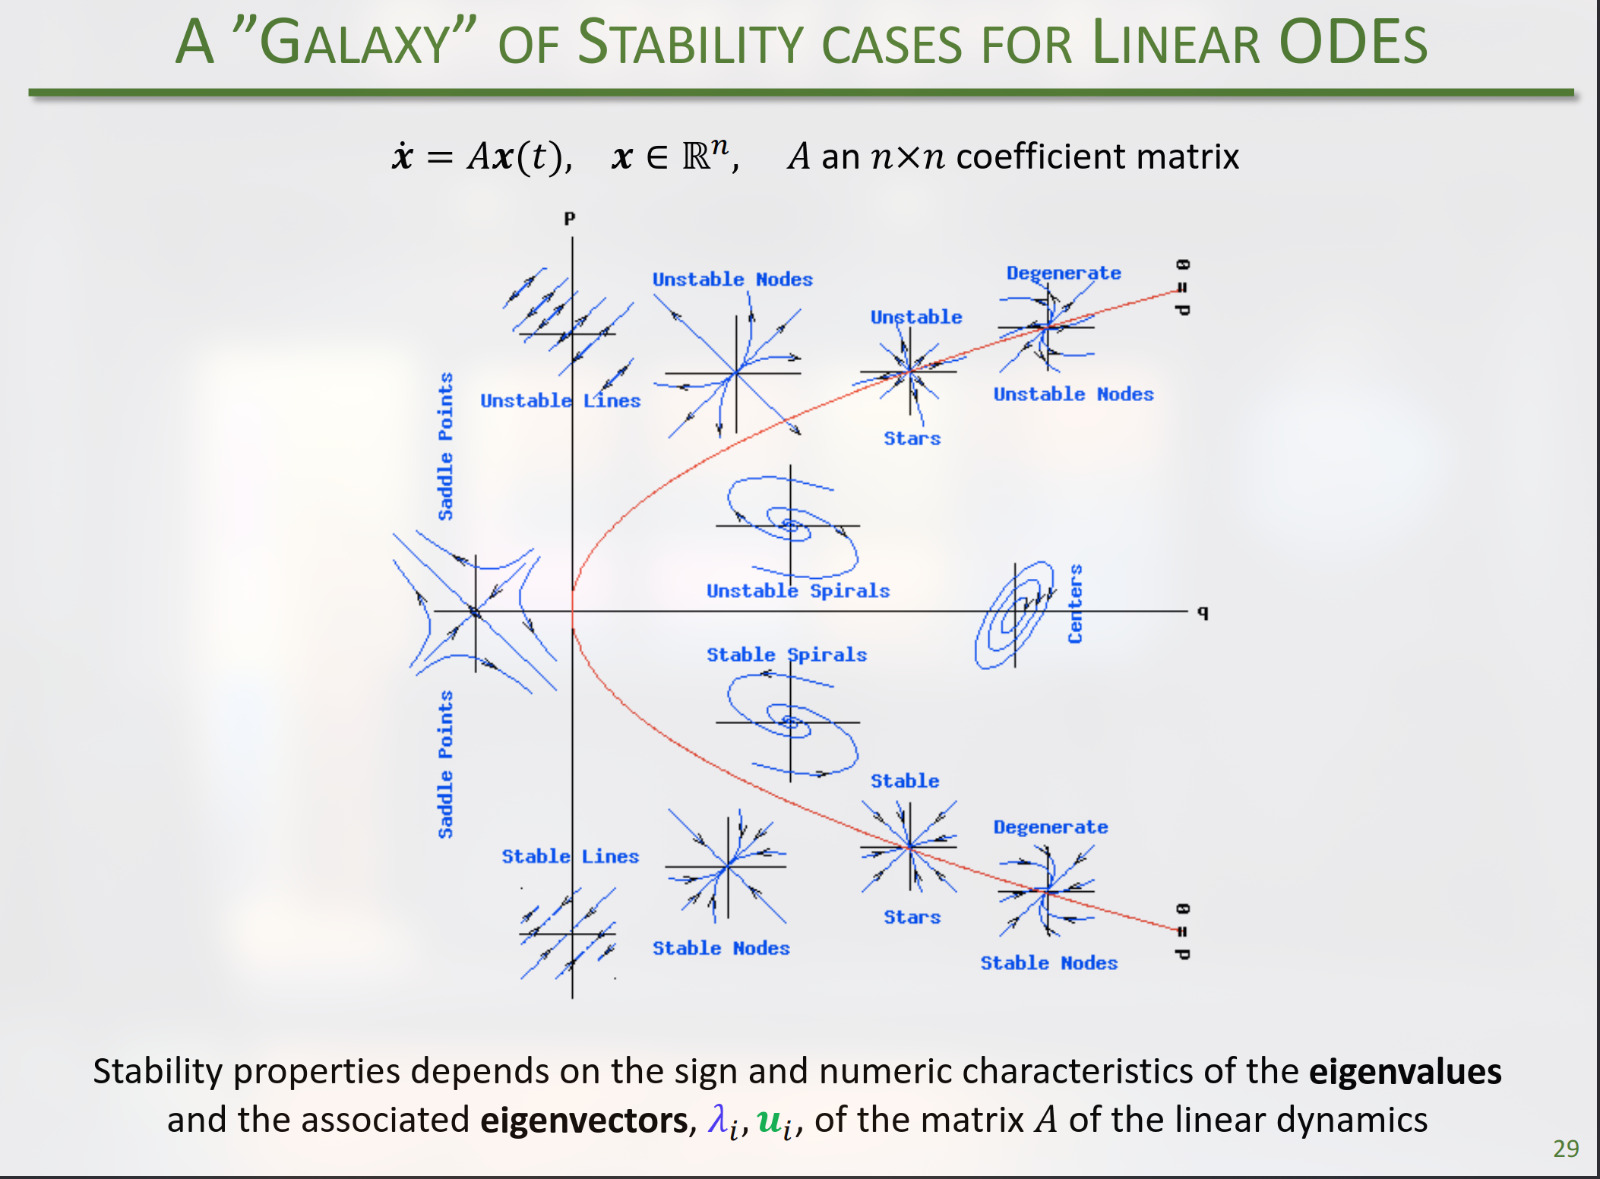
\includegraphics[width=0.6\textwidth]{images/image.png}
\end{center}

\section*{Linear System Classification by Eigenvalues}

% Consider the linear system:
% \[
% \dot{\mathbf{x}} = A\mathbf{x}, \quad A \in \mathbb{R}^{2\times 2}
% \]
% We classify equilibria based on the eigenvalues of \( A \).


% \textbf{1. Two Distinct Real Eigenvalues of Opposite Sign}

% Behavior:
% \begin{itemize}
%   \item Trajectories diverge along one eigenvector and converge along the other.
%   \item Equilibrium is a \textbf{saddle point (unstable)}.
% \end{itemize}

% \textbf{2. Two Distinct Real Eigenvalues with Same Sign}

% Behavior:
% \begin{itemize}
%   \item \textbf{Stable node} if both eigenvalues $< 0$.
%   \item \textbf{Unstable node} if both eigenvalues $> 0$.
%   \item Trajectories are straight lines along eigenvectors.
% \end{itemize}

% \textbf{3. One Repeated Real Eigenvalue, Two Independent Eigenvectors (Star / Proper Node)}

% Behavior:
% \begin{itemize}
%   \item Repeated real eigenvalue (algebraic multiplicity = 2).
%   \item Two linearly independent eigenvectors.
%   \item Trajectories are straight lines toward/away from the origin.
%   \item \textbf{Stable} if $\lambda < 0$, \textbf{unstable} if $\lambda > 0$.
% \end{itemize}

% \textbf{4. One Repeated Real Eigenvalue, One Eigenvector (Improper / Degenerate Node)}

% Behavior:
% \begin{itemize}
%   \item Repeated real eigenvalue with only one eigenvector.
%   \item Requires a generalized eigenvector.
%   \item Trajectories are curved, tangent to the direction of the eigenvector.
%   \item \textbf{Stable} if $\lambda < 0$, \textbf{unstable} if $\lambda > 0$.
% \end{itemize}

% \textbf{5. Complex Eigenvalues with Nonzero Real Part (Spiral / Focus)}

% \[
% A =
% \begin{pmatrix}
% a & -b\\
% b & a
% \end{pmatrix}, \quad
% \lambda_{1,2} = a \pm bi
% \]

% \[
% \mathbf{x}(t) = e^{at}
% \begin{pmatrix}
% \cos(bt) & -\sin(bt)\\
% \sin(bt) & \cos(bt)
% \end{pmatrix}
% \mathbf{x}(0)
% \]

% \textbf{Behavior:}
% \begin{itemize}
%   \item Complex conjugate eigenvalues.
%   \item \textbf{Stable spiral} if $a < 0$, \textbf{unstable spiral} if $a > 0$.
%   \item Trajectories rotate while exponentially approaching or diverging from origin.
% \end{itemize}

% \textbf{6. Pure Imaginary Eigenvalues (Center)}

% \[
% A =
% \begin{pmatrix}
% 0 & -\omega\\
% \omega & 0
% \end{pmatrix}, \quad
% \lambda_{1,2} = \pm i\omega
% \]

% \[
% \mathbf{x}(t) =
% \begin{pmatrix}
% \cos(\omega t) & -\sin(\omega t)\\
% \sin(\omega t) & \cos(\omega t)
% \end{pmatrix}
% \mathbf{x}(0)
% \]

% \textbf{Behavior:}
% \begin{itemize}
%   \item Purely imaginary eigenvalues, no real part.
%   \item Trajectories are closed orbits (circles or ellipses).
%   \item Neither converge nor diverge — \textbf{neutrally stable}.
% \end{itemize}

(for the saddle case, keep in mind a product is negative only
if exaclty one of the numbers is negative)

\renewcommand{\arraystretch}{1.1} % less vertical space
\begin{tabular}{|c|c|c|}
\hline
\textbf{Eigenvalues} & \textbf{Critical Point} & \textbf{Stability} \\
\hline
$r_1, r_2 > 0$ & Node (real, distinct) & Unstable \\
$r_1, r_2 < 0$ & Node (real, distinct) & Asymptotically stable \\
$r_1 r_2 < 0$ & Saddle & Unstable \\
$r_1 = r_2 \neq 0$ & Node / Improper node & Same as sign of $r_1$ \\
$r_{1,2} = \lambda \pm i\mu$ & Spiral (focus) & Same as sign of $\lambda$ \\
$r_{1,2} = \pm i\mu$ & Center & Neutrally stable \\
\hline
\end{tabular}

\section*{Perturbations}

For Pure Imaginary Eigenvalue,
small perturbations add a tiny real part to the eigenvalues:

\begin{itemize}
    \item $\lambda > 0$ (positive real part) $\implies$ trajectories spiral outward (unstable spiral).
    \item $\lambda < 0$ (negative real part) $\implies$ trajectories spiral inward (stable spiral).
\end{itemize}

For Repeated Real Eigenvalues

\begin{itemize}
    \item If the eigenvectors are linearly independent, the system stays a node, but may change to a saddle if the signs differents.
    \item If the eigenvectors are linearly dependent (a degenerate node),
    a small perturbation will typically turn it into either a spiral
    (if eigenvalues become complex) or a node
    (if eigenvalues become distinct real numbers).
\end{itemize}

\section*{Linearization around a Critical Point}

Consider a nonlinear system:
\[
\dot{\mathbf{x}} = \mathbf{f}(\mathbf{x}), \quad \mathbf{x} \in \mathbb{R}^n
\]

Let $\mathbf{x}_0$ be a critical point: $\mathbf{f}(\mathbf{x}_0) = 0$.

\textbf{Step 1: Linear Approximation}

\[
\mathbf{f}(\mathbf{x}) \approx \mathbf{f}(\mathbf{x}_0) + J_{\mathbf{f}}(\mathbf{x}_0)(\mathbf{x} - \mathbf{x}_0)
\]

Since $\mathbf{f}(\mathbf{x}_0) = 0$, the linearized system is
\[
\dot{\mathbf{x}} \approx J_{\mathbf{f}}(\mathbf{x}_0) (\mathbf{x} - \mathbf{x}_0), \quad
\mathbf{y} = \mathbf{x} - \mathbf{x}_0
\]

\textbf{Step 2: Jacobian Matrix}

\[
J_{\mathbf{f}}(\mathbf{x}_0) =
\begin{bmatrix}
\frac{\partial f_1}{\partial x_1} & \cdots & \frac{\partial f_1}{\partial x_n} \\
\vdots & \ddots & \vdots \\
\frac{\partial f_n}{\partial x_1} & \cdots & \frac{\partial f_n}{\partial x_n}
\end{bmatrix}_{\mathbf{x} = \mathbf{x}_0}
\]

\textbf{Step 3: Eigenvalues, Eigenvectors, and General Solution}

Compute eigenvalues $\lambda_i$ and eigenvectors $\mathbf{v}_i$ of $J_{\mathbf{f}}(\mathbf{x}_0)$.
The general solution of the linearized system is
\[
\mathbf{y}(t) = \sum_{i=1}^n c_i e^{\lambda_i t} \mathbf{v}_i, \quad
\mathbf{x}(t) = \mathbf{x}_0 + \mathbf{y}(t)
\]

\textbf{Step 4: Stability Analysis}

Stability is determined by the eigenvalues of the Jacobian $J_{\mathbf{f}}(\mathbf{x}_0)$, just like in the linear case.

\section*{Global Behavior and Nullclines}

\begin{itemize}
  \item \textbf{Basin of Attraction:} The set of all initial conditions that eventually lead a trajectory to the same stable equilibrium point.
  \item \textbf{Separatrix:} The boundary between different basins of attraction.
  \item \textbf{Isoline:} The set of points where a function takes the same value.
  \item \textbf{Isocline:} The set of points where the vector field has the same \textbf{slope}.
  \item \textbf{Nullcline:} A specific type of isocline. It's the set of points where the slope is either zero or infinite (i.e., where one component of the vector field is zero).
\end{itemize}

Nullcline fun facts:
\begin{enumerate}
  \item The \textbf{$x$-nullcline} is the curve where $\dot{x} = f(x,y) = 0$.
  \item The \textbf{$y$-nullcline} is the curve where $\dot{y} = g(x,y) = 0$.
  \item On the $x$-nullcline, the vector field has no horizontal component, so vectors can only point vertically (up or down).
  \item On the $y$-nullcline, the vector field has no vertical component, so vectors can only point horizontally (left or right).
  \item \textbf{Equilibrium points} are exactly at the intersection of the $x$-nullclines and $y$-nullclines (since $\dot{x}=0$ and $\dot{y}=0$ simultaneously).
  \item Nullclines divide the phase space into regions. In each region, the sign of $\dot{x}$ and $\dot{y}$ is constant.
\end{enumerate}

\section*{Limit cycles}

\textbf{A periodic orbit} is just any trajectory that forms a closed loop.

\textbf{A limit cycle} is an isolated closed trajectory.
This means neighboring trajectories are not closed; they either spiral into the limit cycle (a stable limit cycle) or spiral away from it (an unstable limit cycle).
There's also mixed scenarios (half-stable)

Example: Van der Pol Oscillator

\section*{2D is Boring}

\begin{theorem}
Any closed trajectory muyst encolse at least one equilibrium
\end{theorem}
\begin{theorem}{Poincare-Bendixson Theorem:}

IF a trajectory is trapped in a closed, bounded region R,

AND this region R contains no equilibrium points,

THEN the trajectory must eventually approach a limit cycle.
\end{theorem}

In other words, 2D systems cannot have chaos

\section*{Chaos and Strange Attractors}

3 main types of attractors: Fixed Points, Limit Cycles and Strange Attractors (the last
appears only in 3D+)

Properties of strange attractors:
\begin{itemize}
  \item Sensitive dependence on initial conditions: two initial conditions very
  close to each other become very far apart as time goes on (but remain confined in the set
  that defines the attractor)
  \item Fractal dimensions (e.g. $2.06$). Non-integer
\end{itemize}

\textbf{Example: Lorenz Attractor}
\begin{enumerate}
  \item For a parameter r=21, trajectories spiral into one of two stable fixed points.
  \item For r=28, the fixed points become unstable. Trajectories are still
  bounded, but they never settle down. They move from one "wing" of the
  attractor to the other in an aperiodic, unpredictable way.
\end{enumerate}

\begin{definition}
Chaos: \textbf{aperiodic long-term behavior} in a \textbf{deterministic} system that exhibits
\textbf{sensitive dependence on initial conditions}
\end{definition}
